\documentclass[article,12pt,onesidea,4paper,english,brazil]{abntex2}

\usepackage{lmodern, indentfirst, nomencl, color, graphicx, microtype, lipsum,textcomp}			
\usepackage[T1]{fontenc}		
\usepackage[utf8]{inputenc}		

\setlrmarginsandblock{2cm}{2cm}{*}
\setulmarginsandblock{2cm}{2cm}{*}
\checkandfixthelayout

\setlength{\parindent}{1.3cm}
\setlength{\parskip}{0.2cm}

\SingleSpacing

\begin{document}
	
	\selectlanguage{brazil}
	
	\frenchspacing 
	
	\begin{center}
		\LARGE QUALIDADE MICROBIOLÓGICA DE PRODUTOS HORTIFRUTIGRANJEIROS COMERCIALIZADO NA FEIRA LIVRE DO MUNICÍPIO DE COLORADO DO OESTE/ RO.\footnote{Trabalho realizado dentro da (área de Conhecimento CNPq/CAPES: microbiologia de Alimentos) com financiamento do (IFRO).}
		
		\normalsize
		Caroline Alves Lima\footnote{Bolsista modalidade PIBITI. E-mail: carolyne.ifro@hotmail.com, Campus Colorado do Oeste.} 
		Matheus Henrique Brandão\footnote{Colaborador, modalidade PIBITI. e-mail: mhbrandao@hotmail.com. Campus Colorado do Oeste.} 
		Nélio Ranieli Ferreira de Paula\footnote{Orientador, modalidade PIBITI. E-mail: nelio.ferreira@ifro.edu.br, Campus Colorado do Oeste.} 
	\end{center}
	
	% resumo em português
	\begin{resumoumacoluna}
	Este estudo foi realizado na feira municipal de Colorado do Oeste/RO, localizado no cone sul do estado de Rondônia, as análises microbiológicas dos alimentos foram realizadas no laboratório de microbiologia de alimentos, do instituto federal de educação, ciências e tecnologia, campus Colorado do Oeste. No qual foram realizadas análises de microrganismos Termotolerantes a 37 e 45 ºC, contagem bacteriana total, Staphilococus aureus, Escherichia coli, e Salmonella sp. Todos os produtos analisados estavam impróprios para o consumo, o que demonstra a necessidade de um maior controle da qualidade dos produtos hortifrutigranjeiros que estão à venda nas feiras livres, de forma não colocar em risco a saúde dos consumidores dos produtos hortifrutigranjeiros.
	
		\vspace{\onelineskip}
		
		\noindent
		\textbf{Palavras-chave}: Microrganismos. Saúde pública. Segurança alimentar.
	\end{resumoumacoluna}
	
	\textual
	
	\section*{Introdução}
	
A feira livre é uma forma de comercio que aproxima o consumidor do comerciante, possui uma identidade própria, e se caracteriza pelo encontro de uma grande variedade de pessoas, consumindo ou comercializando (BOECHAT, P.T.V., SANTOS, J.L. 2009). Atualmente, há grande preocupação do consumidor com a qualidade dos alimentos e com os riscos que eles podem acarretar a saúde, tornando urgente o estabelecimento de padrões obrigatórios de segurança alimentar. (ANDREOTTI, A. 2003).

Devido à falta de higiene-sanitária nas feiras, a comercialização dos alimentos de origem animal e vegetal causam uma série de doenças aos consumidores (FORSYTHE, S. J. 2013). A partir desta problemática, a feira livre do município de Colorado do Oeste-RO possui adequada qualidade higiene-sanitária, sem a qual pode-se acarretar problemas de origem alimentar?

Deste modo, o presente estudo teve como objetivo avaliar a segurança alimentar dos produtos vendidos nas feiras-livres, por meio de analises microbiológicas dos produtos hortifrutigranjeiros.
	
	\section*{Material e Método}
	
Este projeto foi desenvolvido no Instituto Federal de Educação, Ciência e Tecnologia, Campus Colorado do Oeste – RO, Laboratório de análises microbiológicas de produtos agroindustriais utilizando-se metodologia proposta pelo manual de métodos de análise microbiológica de alimentos e água (SILVA, N.et al. 2010) e pela Internacional Comissiono Microbiologic Specification for Foods Method
- ICMSF (1983).

Para tanto, um total de 27 amostras de produtos hortifrutigranjeiros foram coletados na feira municipal de Colorado do Oeste/RO, localizado no cone sul do estado de Rondônia. Desta forma, foram realizadas amostragens aleatórias, para avaliar as condições do lote, qualidade, manipulação e processamento, obtidas através das coletas e análises de produtos de origem vegetal, especificamente: alface, melancia, calda de cana, além de produtos de origem animal, mais precisamente cárneos: carne bovina, suína e peixe; derivado de leite: queijo, iogurte e requeijão. Tais os produtos foram coletados nas bancas aleatoriamente.

Foi utilizado amostras de 25g dos produtos homogeneizados em 225ml de água peptonada 0,1\% (p/v) esterilizada, para realizar todos os testes: Salmonella sp. bactérias Termotolerantes (coliformes totais, fecais e Escherichia sp.).

O teste de bactérias Termotolerantes foi realizado com a inoculação de alíquotas da amostra contendo tubos de Durhan invertidos e Caldo Lauril Sulfato Triptose (LST), incubados a 37oC (totais) por 24 - 48 horas. Os tubos positivos para coliformes apresentaram turvação e formação de gás. Os coliformes a 45oC (fecais) foram quantificados a partir de alíquotas transferidas dos tubos positivos de coliformes a 37oC, com auxílio de uma alça de repicagem, para tubos contendo caldo Escherichia coli (EC) com tubos de Durhan invertidos. Aqueles que apresentarem gás são positivos.

Já para a análise de Salmonela sp. foi utilizado alíquotas dos tubos positivos de coliformes a 37°C. no qual foi utilizado cem microlitros de caldo para cada placa, estas em duplicata, os caldos utilizados para Salmonela sp. foi o Caldo Rappaport- Vassiliadis (RP), as alíquotas foram homogeneizadas nas placas com auxílio de uma alça drigalsck. As placas foram incubadas a 37oC por 48 horas.
	
	\section*{Resultados e Discussão}
	
Dentre estas, bactérias Termotolerantes a 45ºC, Escherichia sp. e Salmonella sp. Os resultados foram quantificados e qualificados para a presença ou ausência dos patógenos.

\begin{figure}[!h]
	\centering
	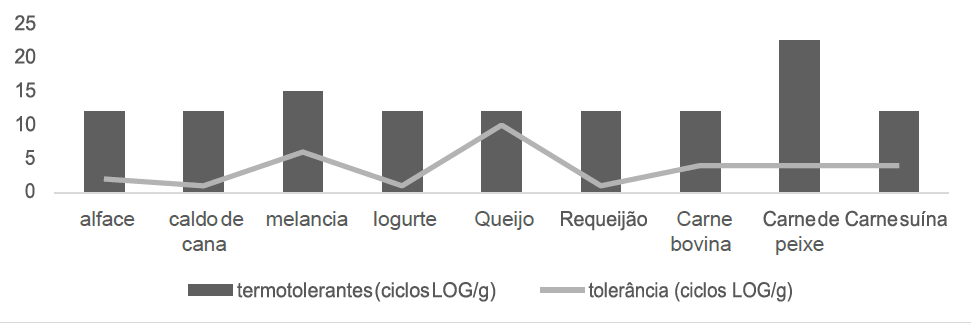
\includegraphics[width=.8\linewidth]{pip-167-01}
	\caption{Resultado da análise microbiológica de Termotolerantes}
\end{figure}

Observa-se que os produtos coletados nas feiras apresentam um elevado grau de contaminação, isto se dá pela curva de tolerância obtidos com as análises e pelo grau de contaminação aceitável pela legislação, sendo esta a Resolução nº 12 da ANVISA. Esta resolução tem como objetivo o estabelecimento dos padrões microbiológicos sanitários para alimentos destinados ao consumo humano. A presença de Termotolerantes em alimentos indica condições adequadas durante o processo, produção ou armazenamento, e altas contagens podem significar contaminação pós-processamento, limpeza e sanitização deficiente, matérias-primas contaminadas (BROD, 2002; MACIEL, 2002).

A Escherichia coli se destaca no cenário nacional e internacional como sendo um microrganismo de importância higiênico-sanitária e saúde pública. (FRANCO, R.M.; MANTILLA, S. P.S.; OLIVEIRA, L. A. T. 2010). Salmonella sp. é outro
microrganismo que também tem grande participação no cenário da segurança alimentar. A salmonelose está entre uma das toxinfecções alimentares mais importantes, sendo que esta doença é causada por bactérias do gênero Salmonella (CARDOSO, T. G. 2006).

As análises de Eschechia coli e Salmonella sp. foram avaliadas por meio da ausência ou presença dos microrganismos.

\begin{table}[h]
	\centering
	\caption{Resultado das análises de Escherichia coli e Salmonella sp}
	\label{my-label}
	\begin{tabular}{p{.3\linewidth}p{.3\linewidth}p{.3\linewidth}}
		\hline
		\multicolumn{3}{c}{Análise de Escherichia coli e Salmonella sp.} \\
		\hline
		Produtos             & Eschechia coli      & Salmonella sp.      \\
		Alface               & ausente             & ausente             \\
		Caldo de cana        & presente            & indicativo          \\
		Melancia             & ausente             & ausente             \\
		Requeijão            & presente            & indicativo          \\
		Iogurte              & presente            & indicativo          \\
		Queijo               & presente            & indicativo          \\
		Carne suína          & ausente             & indicativo          \\
		Carne bovina         & ausente             & indicativo          \\
		Carne de peixe       & ausente             & indicativo         \\ \hline
	\end{tabular}
\end{table}

A partir destes dados pode-se destacar que a maioria dos produtos coletados estavam ausentes para o microrganismo Escherichia coli, exceto os produtos caldo de cana, requeijão, iogurte e queijo que obtiveram presença deste microrganismo.

Com relação a Salmonella sp. visualiza-se que a maioria dos produtos foram rotulados de indicativos, isso se dá devido a formação de uma cor negra que representa a formação de sulfetos, tais organismos desenvolvem colônia dessa forma como Proteus spp. e algumas espécies de Salmonella spp. As bactérias formadoras de sulfetos formam colônias transparentes que apresentam um centro negro (Neogen do Brasil. 2011).

A maioria dos produtos coletados estavam ausentes para o microrganismo Escherichia coli. Entretanto, esta estava presentem nos produtos: caldo de cana, requeijão, iogurte e queijo. Este resultado indica que tais produtos possuem grande chance de causar alguma infecção ao serem ingeridos, uma vez que quando detectada no alimento, esta bactéria indica que o alimento tem uma contaminação
bacteriana de origem fecal e, portanto, apresenta condições higiênico-sanitárias insatisfatórias (FRANCO, B.D.G.H.; LANDGRAF, M. 1996).
	
	\section*{Conclusões}
	
A qualidade destes produtos não está apenas relacionada à manutenção das características sensoriais e ampliação da vida útil dos produtos, mas também no controle da microbiota epífita presente e da microbiota contaminante adquirida desde a colheita até a distribuição ao consumidor. O controle microbiológico dos hortifrutigranjeiros envolve fatores tais como: qualidade da matéria prima, condições de processamento, tipos de embalagem, de armazenamento, e manejo sanitário correto ao longo da cadeia de produção.
	

	\section*{Referências}
	
	\sloppy
	
\noindent ANDREOTTI, A. et. Al. importância do treinamento para manipuladors de aliments em relação a higiene pessoal. Revista Iniciação Científica Cesumar ., v. 05. p. 29 – 33.2003.

\noindent ANVISA - Agência Nacional de Vigilância sanitária. Resolução RDC nº 12, REGULAMENTO TÉCNICO SOBRE PADRÕES MICROBIOLÓGICOS PARA ALIMENTOS. BRASIL. 2000.

\noindent BOECHAT, P.T.V., SANTOS, J.L. feira livre: dinâmicas especiais e relações indenitárias. Anais... SP. 2009.

\noindent BROD, F.C.A. et al. Avaliação das condições higiênico-sanitárias de lanches comercializados em vias públicas em cidades da fronteira noroeste/RS. Anais... RS. 3685p. 2002.

\noindent FORSYTHE, S.J. Microbiologia dos alimentos. 2 ed.- Porto alegre: Artmed, 2013. FRANCO, B.D.G.H.; LANDGRAF, M. microbiologia de alimentos. São Paulo:
Atheneu. 1996, 181 p.

\noindent FRANCO, R. M.; MANTILLA, S. P.S.; OLIVEIRA, L. A. T. Viabilidade de Escherichia coli patogênica em linguiça frescal suína. Revista Acadêmica: Ciências Agrárias e Ambientais. Curitiba, v. 8, n. 3, p. 319-325. 2010.

\noindent Neogen do Brasil. ÁGAR SALMONELLA SHIGELLA – SALMONELLA SHIGELLA AGAR (7152). SP. 2011.
SILVA, N.et al. Manual de métodos de análise microbiológica de alimentos e agua. 4 ed. – São Paulo: livraria varela, 2010.

	
\end{document}
